\documentclass[11pt]{article}

% A hack to make deauthor not complain which redefines
% the titlepage command
% \newcommand{\titlepage}{}

\usepackage{deauthor,times,graphicx}

% JobGraph and Execution figs
\usepackage{tikz}
\usetikzlibrary{arrows,automata,calc,positioning,shapes.geometric}

% trademark symbol
\usepackage{textcomp}

% code listings
\usepackage{listings}

\definecolor{dkgreen}{rgb}{0,0.6,0}
\definecolor{gray}{rgb}{0.5,0.5,0.5}
\definecolor{mauve}{rgb}{0.58,0,0.82}

% there is no built in support or Scala yet, good enough
\lstset{frame=tb,
  language=Java,
  aboveskip=3mm,
  belowskip=3mm,
  showstringspaces=false,
  columns=flexible,
  basicstyle={\scriptsize\ttfamily},
  numbers=none,
  numberstyle=\tiny\color{black},
  keywordstyle=\color{blue},
  commentstyle=\color{dkgreen},
  stringstyle=\color{mauve},
  breaklines=true,
  breakatwhitespace=true,
  tabsize=4,
  %for scala
  emph={%  
    object, def, val, zip%
    },emphstyle={\color{blue}}%
}%

% url references
\usepackage{hyperref}

% in paragraph enums
\usepackage{paralist}

\begin{document}



\title{Apache Flink\texttrademark : Streaming dataflows as a basis for universal data analytics}
\author{Authors}

\maketitle

\begin{abstract}
Abstract TBD.
\end{abstract}


\section{Introduction}

Organizations rely more and more on the value of their data, which is directly correlated with its freshness. In addition, as the data infrastructure becomes more and more complex, development time is focused on integrating different systems together, rather than focusing on business logic. The ever-growing need for lower latency analytics and scale, creates a pressing need for more real-time, asynchronous, data processing infrastructure.

Various real-time analytics and CEP tools are currently in use by the industry, including TIBCO, IBM Infosphere Streams, Microsoft Streaminsight, Streambase, etc. These systems implement and extend the results of research which has been done in the database community in the last 15 years, with projects such as Aurora, Telegraph, STREAMS, etc. However, the era of Web-scale computing, spawned the development of internal ``roll-your-own'', solutions based on systems like Apache Storm, Samza, Kafka, Spark, etc. These systems provide very low level APIs and enforce only custom, application-specific solutions to be built on top.  Moreover, in the lack of better solutions, the industry is using traditional batch processing platforms to serve streaming use cases. This has led to approaches such a ``micro-batching''~\cite{Zaharia:2013:DSF:2517349.2522737}, where a batch processor is used to simulate continuous processing, and the ``lambda architecture''~\cite{marz2015big}, where a stream processor is aided by a batch processor to compensate for lack of performance and consistency guarantees.

We believe that there is still a need for a real-time analytics platform, that is not covered by the existing solutions described above. Our observation is that modern enterprises need a platform that integrates well in the Hadoop-related Big Data processing zoo, supports user-defined computations, while being able to perform efficient, scalable and consistent data analysis, on top of both streaming/unbounded and stored/batch data.

Apache Flink is a platform that was designed to deliver on these requirements. It is an open source project licensed by the Apache Software Foundation (ASF)~\cite{CUSTOM:web/Apache}, with its community counting more than 120 developers, and growing fast.~\cite{CUSTOM:web/FlinkContrib} Flink originates from the database research community, in particular the Stratosphere research project~\cite{stratosphere}, and incorporates several novel research contributions, some of which have been published in research venues in the past, and some of which have only been published in the form of blog posts or wiki pages. In this article, we attempt a short description of the architecture of the system, highlighting its novel aspects.

This paper is organized as follows: Section X presents a novel paradigm for distributed dataflows based on the notions of operators and logical intermediate results. Section Z presents a novel mechanism to provide fault tolerance while keeping the latency low and the throughput high. Section Y presents methods to overcome limitations of the JVM by careful engineering, and how to while extend cost-based optimization to user-defined functions~\cite{battre2010nephele, DBLP:journals/pvldb/EwenTKM12} and efficiently embed iterations within a DAG-based dataflow system~\cite{DBLP:journals/pvldb/EwenTKM12}. 


\section{System architecture}

In this section we lay out the architecture of Flink as a software stack, and as a distributed system. While Flink's stack of APIs continues to grow, we can distinguish four main layers: deployment, core, APIs, and libraries.

\begin{figure}[h!]
	\centering  	
  	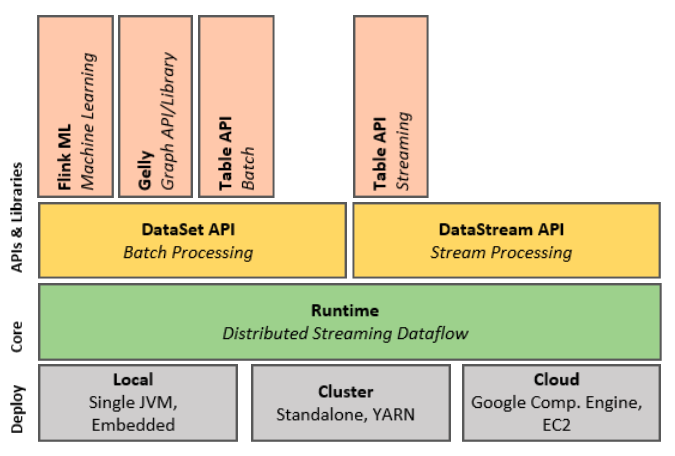
\includegraphics[width=.45\textwidth]{figs/flink_stack.png}
	\caption{The Flink software stack.}
	\label{fig:FlinkStack}
\end{figure}

\textbf{Flink's Runtime and APIS.} The core of Flink is the distributed dataflow engine, which executes dataflow programs called Job Graphs. A Job Graph is a DAG of operators and connections between operators. There are two ``core'' APIs in Flink: the DataSet API for processing finite data sets (often referred to as ``batch processing''), and the DataStream API for processing potentially unbounded data streams (often referred to as ``stream processing''). Flink's core runtime engine can be seen as a streaming dataflow engine, and both the DataSet and DataStream APIs create programs (Job Graphs) accepted by this engine. On top of the core APIs, Flink bundles ``domain-specific'' libraries and APIs that generate DataSet and DataStream API programs. Currently these are the following:
\begin{inparaenum}[i)]
  \item Gelly, an API and library for processing graphs,
  \item FlinkML, an API and library for composing Machine Learning pipelines and
  \item Table, an API similar in spirit to Microsoft's LINQ.
\end{inparaenum}
A Flink cluster comprises of three types of processes: the client, the JobManager, and the TaskManager. The client takes the program code (written in a mixture of Flink's APIs), transforms it to a Job Graph, and submits it to the JobManager. The compilation process involves a type extraction and checking phase that generates serializers and comparators for all used types. DataSet programs, also go through a cost-based query optimization phase, similar to the physical optimizations performed by relational query optimizers (more details in Section X).

The JobManager is Flink's master node. It coordinates all message-passing during job execution by sending heartbeats to the TaskManagers, receiving statistics, controls the tasks' lifecycle,  coordinates the fault tolerance machanisms. The actual data processing takes place in the TaskManagers, or worker processes that they execute several tasks in multiple threads, and maintain data structures shared by all tasks (e.g., buffer pools) executed by a TM. TMs communicate directly with each other using a multiplexed TCP connection per TM pair. 


\section{Execution model}

\textbf{The Job Graph.} Flink's execution model is based on the Job Graph, a directed acyclic graph (DAG) that consists of nodes and edges. There are two classes of nodes: (stateful) operators, and (logical) intermediate results (IRs). For example, the graph below consists of five operators ($op_1$-$op_5$), and three intermediate results ($ir_1$-$ir_3$). Operators abstract computation (e.g., transformations, joins, etc), state (e.g., a persistent counter), as well as data sources (e.g. reading data from a file system, a socket, a message queue, etc.), and data sinks. Operators produce intermediate results, as well as updates to state. An intermediate result is a logical handle (pointer) to the data that is produced by one operator. An intermediate result can be consumed by one or more operators. Intermediate results are logical in the sense that the data they point to may or may not be materialized on disk.

\begin{figure}[ht]
\centering
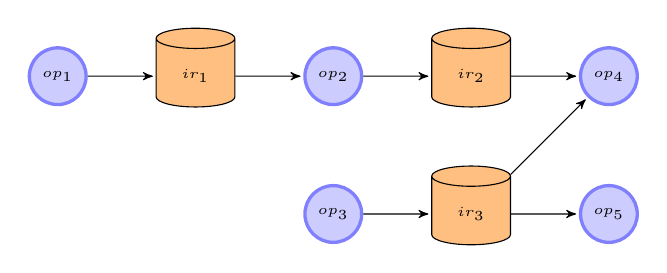
\begin{tikzpicture}
[shorten >=1pt,node distance=1.75cm,>=stealth',initial text=, font=\tiny]
\tikzstyle{op}=[circle, draw=blue!50,very thick,fill=blue!20]
\tikzstyle{ir}=[cylinder, cylinder uses custom fill, cylinder body fill=orange!50, cylinder end fill=orange!50, shape border rotate=90, aspect=0.35, draw, minimum size=1cm, text width=0.5cm, align=center]

\node[op] (op_1) {$op_1$};
\node[ir] (ir_1) [right of = op_1] {$ir_1$};
\node[op] (op_2) [right of = ir_1] {$op_2$};
\node[ir] (ir_2) [right of = op_2] {$ir_2$};
\node[op] (op_3) [below of = op_2] {$op_3$};
\node[ir] (ir_3) [right of = op_3] {$ir_3$};
\node[op] (op_4) [right of = ir_2] {$op_4$};
\node[op] (op_5) [right of = ir_3] {$op_5$};
			
\path[->] 	
			(op_1) 	edge node [above] {} (ir_1)
			(ir_1) 	edge node [above] {} (op_2)
			(op_2) 	edge node [above] {} (ir_2)
			(ir_2) 	edge node [above] {} (op_4)
			(op_3) 	edge node [above] {} (ir_3)
			(ir_3) 	edge node [above] {} (op_4)
			(ir_3) 	edge node [above] {} (op_5)
			;
\end{tikzpicture}
\label{fig:JobGraph}
\caption{The JobGraph is the logical view of a Flink job.}
\end{figure}

\textbf{Parallelized Job Graphs.} When the JobGraph is scheduled in a cluster for execution, it is parallelized to form an ExecutionGraph. An ExecutionGraph consists of tasks (parallel instances of operators), and intermediate result partitions (IRPs), that represent logical partitions of intermediate results corresponding to different partitioning keys. The JobGraph in fig. \ref{fig:JobGraph}, if it is partitioned using a parallelism of two, it results to the ExecutionGraph shown in fig. \ref{fig:ExecutionGraph}. Assume that $op_1$ and $op_2$ are data sources, $op_2$ is a map operator, $op_4$ is a join operator that needs both inputs partitioned by the same key, and $op_5$ is a filter. Assume also that the join is executed as a repartitioned join, i.e., both inputs are partitioned and shuffled over the cluster of 2 nodes (alternatives would be to broadcast one input or leverage a pre-existing partitioning if present). The resulting ExecutionGraph is the following:

\begin{figure}[ht]
\centering
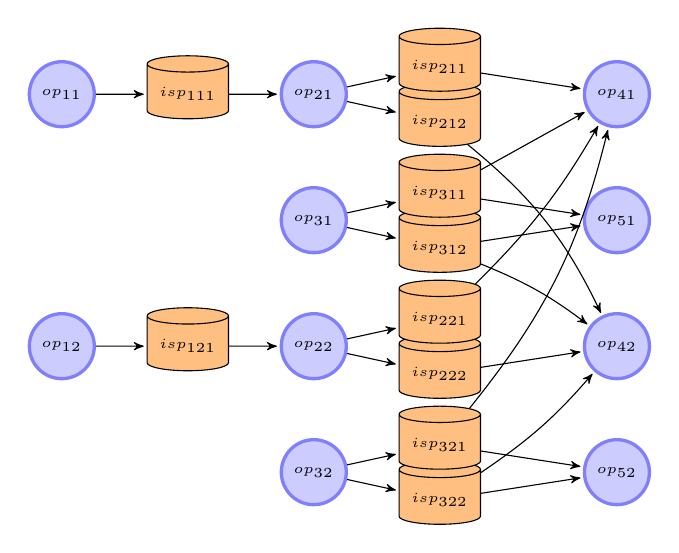
\begin{tikzpicture}
[shorten >=1pt,node distance=1.6cm,>=stealth',initial text=, font=\tiny]
\tikzstyle{every state}=[circle, fill,draw=none,white,text=black]
\tikzstyle{op}=[circle, draw=blue!50,very thick,fill=blue!20]
\tikzstyle{ir}=[cylinder, cylinder uses custom fill, cylinder body fill=orange!50, cylinder end fill=orange!50, shape border rotate=90, aspect=0.2, draw, minimum size=0.8cm, text width=0.8cm, align=center]

\node[op] (op_11) {$op_{11}$};
\node[ir] (isp_111) [right of = op_11] {$isp_{111}$};
\node[op] (op_21) [right of = isp_111] {$op_{21}$};
\node[state] (ir_21) [right of = op_21] {};
\node[ir] (isp_212) [below of = ir_21, node distance = 0.35cm] {$isp_{212}$};
\node[ir] (isp_211) [above of = ir_21, node distance = 0.35cm] {$isp_{211}$};
\node[op] (op_31) [below of = op_21] {$op_{31}$};
\node[state] (ir_31) [right of = op_31] {};
\node[ir] (isp_312) [below of = ir_31, node distance = 0.35cm] {$isp_{312}$};
\node[ir] (isp_311) [above of = ir_31, node distance = 0.35cm] {$isp_{311}$};
\node[op] (op_41) [right of = ir_21, node distance = 2.25cm] {$op_{41}$};
\node[op] (op_51) [right of = ir_31, node distance = 2.25cm] {$op_{51}$};

\node[op] (op_22) [below of = op_31] {$op_{22}$};
\node[ir] (isp_121) [left of = op_22] {$isp_{121}$};
\node[op] (op_12) [left of = isp_121] {$op_{12}$};
\node[state] (ir_22) [right of = op_22] {};
\node[ir] (isp_222) [below of = ir_22, node distance = 0.35cm] {$isp_{222}$};
\node[ir] (isp_221) [above of = ir_22, node distance = 0.35cm] {$isp_{221}$};
\node[op] (op_32) [below of = op_22] {$op_{32}$};
\node[state] (ir_32) [right of = op_32] {};
\node[ir] (isp_322) [below of = ir_32, node distance = 0.35cm] {$isp_{322}$};
\node[ir] (isp_321) [above of = ir_32, node distance = 0.35cm] {$isp_{321}$};
\node[op] (op_42) [right of = ir_22, node distance = 2.25cm] {$op_{42}$};
\node[op] (op_52) [right of = ir_32, node distance = 2.25cm] {$op_{52}$};

			
\path[->] 	
			(op_11) 	edge node [above] {} (isp_111)
			(isp_111) 	edge node [above] {} (op_21)
			(op_21) 	edge node [above] {} (isp_211)
			(op_21) 	edge node [above] {} (isp_212)
			(isp_211) 	edge node [above] {} (op_41)
			(isp_212) 	edge [bend left = 12.5] node [above] {} (op_42)
			(op_31) 	edge node [above] {} (isp_311)
			(op_31) 	edge node [above] {} (isp_312)
			(isp_311) 	edge node [above] {} (op_41)			
			(isp_311) 	edge node [above] {} (op_51)
			(isp_312) 	edge node [above] {} (op_51)
			(isp_312) 	edge [bend left = 7.5] node [above] {} (op_42)
			
			(op_12) 	edge node [above] {} (isp_121)
			(isp_121) 	edge node [above] {} (op_22)
			(op_22) 	edge node [above] {} (isp_221)
			(op_22) 	edge node [above] {} (isp_222)
			(isp_221) 	edge [bend right = 7.5] node [above] {} (op_41)			
			(isp_222) 	edge node [above] {} (op_42)
			(op_32) 	edge node [above] {} (isp_321)
			(op_32) 	edge node [above] {} (isp_322)
			(isp_321) 	edge node [above] {} (op_52)
			(isp_321) 	edge [bend right = 12.5] node [above] {} (op_41)
			(isp_322) 	edge node [above] {} (op_52)
			(isp_322) 	edge [bend right = 7.5] node [above] {} (op_42)
			;
\end{tikzpicture}
\label{fig:ExecutionGraph}
\caption{The ExecutionGraph is the physical view of a Flink job.}
\end{figure}

\textbf{Data Transfer.} The unit of data transfer in the Flink runtime is a buffer. Buffers contain one or more records, and a record can span multiple buffers. Buffers are requested and relinquished from local buffer pools, shared among operators that live in the same task manager. An IRP is simply a collection of buffers. Work in Flink progresses (i.e., records flow through the pipeline) as long as there are buffers available, essentially implementing distributed blocking queues (the logical streams) with bounded capacity (the amount of memory available to the buffer pools, which can be configured by the user). This mechanism, in addition to implementing record network transfers doubles down as a natural way to backpressure the flow in the case of slow operators (including external systems that consume data). 

We mentioned that the intermediate results are logical handles to the data, rather than the data itself. Internally, intermediate results are abstract classes with many implementations. These implementations can perform pipelined data exchange, and blocking data exchange.

\textbf{Pipelined Data Exchange.} Pipelining (also called intra-operator parallelism), means that a producing and a consuming operator make progress at the same time, without the consumer waiting for the producer to finish. Pipelining is required in streaming systems, and is also used in batch systems to reduce latency. Flink implements pipelining by implementing intermediate results which activate network transfers between the producer task and consumer task,  as soon as their first buffer is available. Flink allows the configuration of its buffers' size and timeout. A buffer is sent to its consumer task as soon it is filled,  or as soon as a timeout is reached. Hence, by setting the buffer size and/or timeout to lower values, one can reduce latency, while achieving the opposite effect (i.e., high throughput) by using higher values.

\textbf{Blocking Data Exchange.} Sometimes it is desirable to break a job into stages, scheduling and executing each stage individually (e.g., to enable interactive processing, and better staging of resources in large batch jobs). To do that, the system has to materialize intermediate results (in memory or disk). Flink implements blocking data exchange via an intermediate result that signals its availability only when all the buffers from the producer have been materialized. The cached buffers can double down as a materialized reusable intermediate result. 


\section{Fault Tolerance via \\ Asynchronous Snapshots}

Fault tolerance in Flink is achieved by taking a snapshot of the execution graph at regular intervals. When failure occurs the state of the execution is restored from the latest snapshot. Upon recovery, in order to guarantee exactly-once processing semantics, the records (events) consumed since the latest snapshot are reprocessed in the same order at each respective source. Normally this possible by using persistent message queueing systems, e.g. Apache Kafka.~\cite{CUSTOM:web/Kafka}

Flink's core mechanism for distributed snapshots is called ``Asynchronous Barrier Snapshotting'' (ABS).~\cite{carbone2015lightweight} It creates a global snapshot by collecting the state of each task in the execution graph in an asynchronous manner. It does so by superimposing snapshotting using injected markers, called ``barriers'', in the input data stream. Similar to Chandy-Lamport distributed snapshots~\cite{chandy1985distributed}, the barriers in ABS dictate the records that should be fully processed before each respected global snapshot, however, no records in transit are included in a snapshot, keeping the persisted state at a minimum. ABS achieves this by a special ``aligning'' phase which ensures that all records from all upstream tasks preceding broadcasted barriers have been fully consumed before processing the data stream further. Recovery from failure reverts the execution graph to the most recent snapshot and is fully consistent by respecting the causal dependency of records. Furthermore, ABS~\cite{carbone2015lightweight} supports snapshotting of cyclic graphs.  The operation of ABS is fully decoupled from the backend used for persisting states, thus, allowing multiple different backend implementations to be integrated. The following figure illustrates the snapshot process.

\begin{figure}[h!]
	\centering  	
  	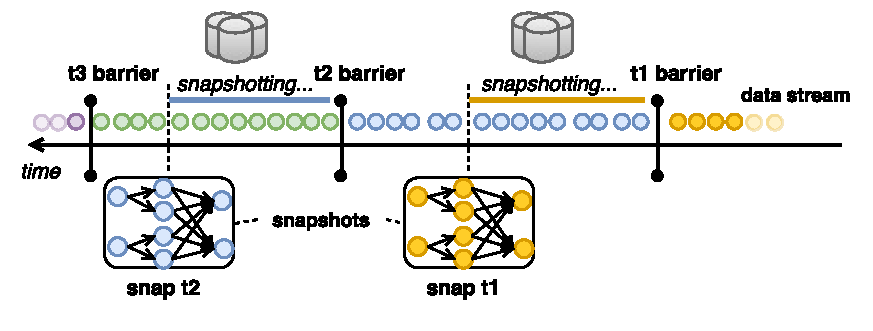
\includegraphics[width=.45\textwidth]{figs/snaps.pdf}
	\caption{Asynchronous Barrier Snapshotting.}
	\label{fig:FlinkStack}
\end{figure}


\section{Stream analytics on top of \\ dataflows}

Flink's DataStream API implements a full stream analytics framework on top of Flink's runtime, including the mechanisms to manage time (including out-of-order event processing), defining windows, and maintaining and updating user-defined state. The streaming API is based on the notion of a DataStream, a (possibly unbounded) immutable collection of elements of a given type. Since the Flink runtime already has pipelined data transfers, continuous stateful operators, and a fault tolerance mechanism for consistent state updates, overlaying a stream processor on top of it essentially boils down to implementing a windowing system and a state interface.The programming model of Flink's streaming API,  builds on two basic abstract data types, namely data streams and window streams. Each of the two supports specific operations since they exhibit different properties. For example, windows support transformations that are only possible on bounded collections such as joins, groupings and aggregations. Other transformations, such as (flat)map are  can be applied incrementally on data streams.

% Give an example here instead of simplicity
The API is designed with simplicity in mind, while at the same time providing powerful tools to deal with time and uncertainty. Here is, for example, a word count program on a simple  time-based window:

\lstinputlisting[label=list:WindowWordCount,caption=WindowWordCount Scala implementation,language=Java]{src/wwc.scala}

Flink distinguishes between two notions of time: 
\begin{description}
\item[Event time] is the time that an event actually happened (e.g., the time that a sensor emitted a signal, or the time that a person tapped on their smartphone).
\item[Processing time] is the wall-clock time of the machine that is processing the data.
\end{description}

In distributed systems, there is an arbitrary lag between event-time and processing-time.~\cite{akidau2015dataflow} This may mean arbitrary delays for getting an answer based on event-time semantics. To avoid arbitrary delays these systems regularly insert special events called ``low watermarks''  that include a time attribute $t$ indicating that all events lower than $t$ have already entered the system. The watermarks aid the execution engine to process events in the correct event order. 

Flink programs that are based on processing time, rely on the machine clocks, and hence a less reliable notion of time, but exhibit the best latency. Programs that are based on event time provide the most reliable semantics, but may exhibit latency due to event time-processing time lag. Flink includes a third notion of time as a special case of event time called ingestion time, which is the time that events enter the system. This provides  a lower latency than event-time semantics, and avoids the arbitrary processing time semantics.

\textbf{Streaming Windows.} A window defines a logical group of records that are processed together. Flink's windowing system largely follows the Dataflow model~\cite{akidau2015dataflow} proposed by Google. A window definition consists of three building blocks: a window assigner, optionally a trigger, and optionally an evictor. 
The assigner predefines the logical groups to which each record belongs, e.g. count-based or time-based periodic windows. The trigger defines when the window operation is performed on each group. The evictor defines which records to keep in each group. The following example defines windows that operate in event time of 6 seconds that slide every 2 seconds (Assigner). The window results are computed once the watermark passes the end of the window (Trigger). Flink also offer short hands for commonly used functionalities.

\lstinputlisting[label=list:GenWindow,caption=Window API functionalities,language=Java]{src/genwin.scala}

A global window creates a single logical group. The following example defines a global window (assigner) that invokes the operation on every 1000 events (trigger) while keeping the last 100 elements (evictor). 

\lstinputlisting[label=list:GlobalWindow,caption=Global Window usage,language=Java]{src/glowin.scala}

Note that streams are already partitioned on a key before windowing, so the above is a local operator that does not require coordination between machines. This mechanism can be used to implement a wide variety of windowing functionality~\cite{akidau2015dataflow}, and Flink comes bundled with syntactic sugar for the most common window definitions (e.g., time- and count-based windows). 

Simple programs in Flink's DataStream API looks like functional, side effect-free programs consisting of transformations on unbounded immutable collections. We incorporate mutable state in the API by providing interfaces to users to register any local variable within a transformation with the system's checkpointed mechanism and freely use this variable in their code. 


\section{Batch analytics on top of \\ dataflows}

A bounded data set is a special case of an unbounded data stream. Thus, a streaming program that inserts all of its input data in a window can form a ``batch`` program and ``batch analytics``, or ``batch processing`` should be fully covered by Flink's features that we presented above. However, \begin{inparaenum}[i)]
  \item the syntax, i.e., the API for batch computation can be simplified (not need for window definitions, simpler joins and loops),
  \item we can simplify the fault tolerance mechanisms and
  \item we can apply query optimization borrowing ideas from MPP database systems.
\end{inparaenum}
For these reasons, Flink treats specially batch computations, by implementing the above optimizations. For enabling batch computations on top of it's streaming runtime, Flink embeds blocking versions of its operators (sorts, joins, etc) within its runtime. These operators simply block until they have received all of their input. Moreover, Flink currently disables the asynchronous snapshotting mechanism for batch programs, and simply uses backtracking based recovery as first described in Dryad.~\cite{isard2007dryad}

With these established, we look that the batch-specific optimizations mentioned above: query optimization, and query processing on paged (managed) memory.

\textbf{Query Optimization.} Flink's optimizer builds on techniques from parallel database systems such as plan equivalences, cost models and interesting properties. However, the arbitrary UDF-heavy DAGs that make up Flink's dataflow programs, do not allow a traditional optimizer to employ database techniques out of the box [black-boxes], since the operators hide their semantics from the optimizer. For the same reason, cardinality and cost estimation methods are equally difficult to employ. Flink's optimizer employs a number of novel methods for overcoming these issues~\cite{blackBoxes, stratosphere, DBLP:journals/pvldb/EwenTKM12} for which we provide a short overview below. Flink's runtime supports various execution strategies including repartition/broadcast data transfer, as well as sort-based grouping and sort- and hash-based join implementations. Flink's optimizer enumerates different physical plans based on the concept of interesting properties propagation~\cite{scopeOptimizer}, using a cost-based approach to choose among multiple physical plans. The cost includes network/disk I/O and CPU cost. To overcome the cardinality estimation issues that were mentioned earlier, Flink's optimizer uses hints that are provided by the programmer.

\textbf{Memory Management.} Building on database technology, Flink, instead of storing objects in the JVM's heap, serializes objects into a  memory segments. These memory segments resemble database blocks into which, Java objects representing the tuples that go through the runtime are serialized. Operations such as sorting, and joining, operate as much as possible on the binary data, keeping the de/serialization overhead at a minimum and partially spilling data to disk when needed. To handle arbitrary objects, Flink uses type inference, and  custom serialization mechanisms.  By keeping the data processing on binary representation and off-heap, Flink manages to reduce the garbage collection overhead, and implement cache-efficient and robust algorithms that scale gracefully in under memory constraints.

\textbf{Native Iterations on top of Dataflows.} The final aspect of Flink on which we focus, is how to implement loops on top of the Flink's dataflow engine. Some approaches execute iterations by submitting new jobs for each iteration or by adding additional nodes to a running DAG~\cite{DBLP:journals/pvldb/BuHBE10, DBLP:conf/hotcloud/ZahariaCFSS10}, hiding from  the engine that it is executing an iterative program. The approach, implemented in Naiad~\cite{murray2013naiad} adds feedback edges in the dataflow graph, supporting graphs with cycles, that  allow for nested iterations. A third approach was to design specialized engines around iterative processing along (e.g., Apache Giraph, and GraphLab) allowing to reduce the number of computations in each iteration.~\cite{low2012distributed}

Flink follows an approach that maintains the DAG-based runtime, but allows for special ``head'' and ``tail'' tasks to signify the beginning and end of iteration, that exchange data via shared memory. This approach simulates a cyclic dataflow within a DAG engine making Flink competitive with specialized graph engines [], while outperforming the driver-based approach []. Flink supports delta iterations [], which exploit sparse computational dependencies, and are used, as the basis for Gelly, Flink's Graph API. Finally, Flink offers Bulk Synchronous Parallel (BSP) iterations in its DataSet API, and asynchronous iterations in its DataStream API.


\section{Related work}

There is, by now, a wealth of engines for distributed batch and stream analytical processing. We categorise these systems below. 

\textbf{Batch Processing.} Apache Hadoop~\cite{CUSTOM:web/Hadoop} is the most popular open source system for large-scale data analysis that is based on the MapReduce paradigm~\cite{DBLP:journals/cacm/DeanG08}. Dryad~\cite{dryad}, introduced embedded user-defined functions in general DAG-based dataflows and was used by SCOPE~\cite{scopeOptimizer} which added a language and an SQL optimizer on top of it. Apache Tez~\cite{CUSTOM:web/Tez} can be seen as an open source implementation of the ideas proposed in Dryad. MPP databases [], and recent open-source implementations~\cite{CUSTOM:web/Drill} [Impala] restrict their API to SQL variants. Very similar to Flink, Apache Spark~\cite{CUSTOM:web/Spark} is a very popular data processing framework that implements a DAG-based processing framework, provides an SQL optimizer, performs driver-based iterations, and treats stream computations as micro-batches. In contrast, Flink is the only system that
\begin{inparaenum}[i)]
  \item supports an optimizer that can optimize DAG programs beyond SQL queries,
  \item is able to perform very efficient iterative processing natively,
  \item includes stream processing as a first-class citizen, enabling more complex use cases than micro-batches.
\end{inparaenum}

\textbf{Stream Processing.} There is a wealth of work on streaming systems, that includes commercial systems like StreamBase, Microsoft StreamInsight, and IBM InfoSphere Streams. Many of these systems are based on research in the database community in projects such as Telegraph [], Aurora/Borealis~\cite{abadi2005design}, Stanford STREAM~\cite{arasu2004stream}, Trill~\cite{chandramouli2014trill} and IBM System S~\cite{chandramouli2014trill}. Most of the above systems are either
\begin{inparaenum}[i)]
  \item academic prototypes,
  \item closed-source commercial products,
  \item do not scale the computation horizontally on clusters of commodity servers.
\end{inparaenum}
Newer open source streaming systems that scale horizontally, such as Apache Storm~\cite{CUSTOM:web/Storm} and Apache Samza~\cite{CUSTOM:web/Samza}, provide low level APIs and offer only at-least-once and at-most-once guarantees. MillWheel~\cite{akidau2013millwheel}, a closed-source system at Google provides exactly-once guarantees with low latency and is used by Google Dataflow~\cite{akidau2015dataflow} to implement  out-of-order stream analytics. To the best of our knowledge, Flink is the only open-source project that
\begin{inparaenum}[i)]
  \item offers high level APIs and processing libraries,
  \item provides state management with exactly-once guarantees and
  \item achieves high throughput and low latency, serving both batch and true streaming computations equally well.
\end{inparaenum}

\section{Conclusion}

In this paper we presented Apache Flink, a platform that implements one universal dataflow engine designed to perform both stream and batch analytics. Flink's dataflow engine treats operator state and logical intermediate results as first class citizens, and is used by the batch and a data stream APIs. The streaming API that is built on top of  Flink's streaming dataflow engine, provides the means to keep recoverable state, and to partition, transform, discretize and aggregate a data stream. While batch computations are, in theory, a special case of a streaming computations, Flink treats them specially, by optimizing their execution with a novel query optimizer, and by implementing blocking operators that gracefully spill to disk in the absence of memory. 

\bibliographystyle{abbrv}
\bibliography{references}

\end{document}